\documentclass[10pt]{article}
\usepackage{graphicx}
\usepackage{multirow}
\usepackage{subcaption}  
\usepackage{multicol}

\usepackage{amsmath}


\usepackage[a4paper, margin=1in, top=0.5in]{geometry}  % Adjust top margin here

\title{Analysis Report: Age Assignment Model Comparison \\ Trust Stamp Assignment}
\author{Pablo Martínez-Agulló}
\date{September 2024}

\begin{document}

\maketitle

\section{Introduction}
Hanut, an online retailer, wants to enhance customer experiences by personalizing them based on age demographics. After exploring image-based age estimation solutions, they have shortlisted two models and are seeking our analysis to determine which model to adopt. Their consumer age profiles are segmented into specific brackets: 0-12, 13-15, 16-17, 18-24, 25-30, 31-40, 41-50, 51-60, 61-70, 71-80, and 81+.

The two shortlisted models are: Model 1, which predicts an age range (\texttt{age\_min} and \texttt{age\_max}) with 6975 entries in \texttt{data/model\_1.csv}, and Model 2, which provides a direct age prediction (\texttt{age}) with 6969 entries in \texttt{data/model\_2.csv}. The ground truth data is stored in \texttt{data/gt.csv} with 8644 entries. Both models' datasets contain some missing entries compared to the ground truth. After merging the datasets, the comparison was performed on 6957 complete entries, with missing data removed.

\section{Data Exploration}
Figure~\ref{fig:Scatter} reveals a trend where both models underestimate age as the real age increases. The $R^2$ value suggests a linear relationship, particularly for Model 1. In all figures, the predictions for Model 1 are represented by the average of \texttt{age\_min} and \texttt{age\_max}. 

The horizontal alignment of points for Model 2 (blue) on Figure~\ref{fig:Scatter} indicates that its predictions might be discretized to specific values instead of providing more granular continuous predictions. The low $R^2$ score of Model 2 may be caused by this.


\begin{figure}[h]
    \centering
    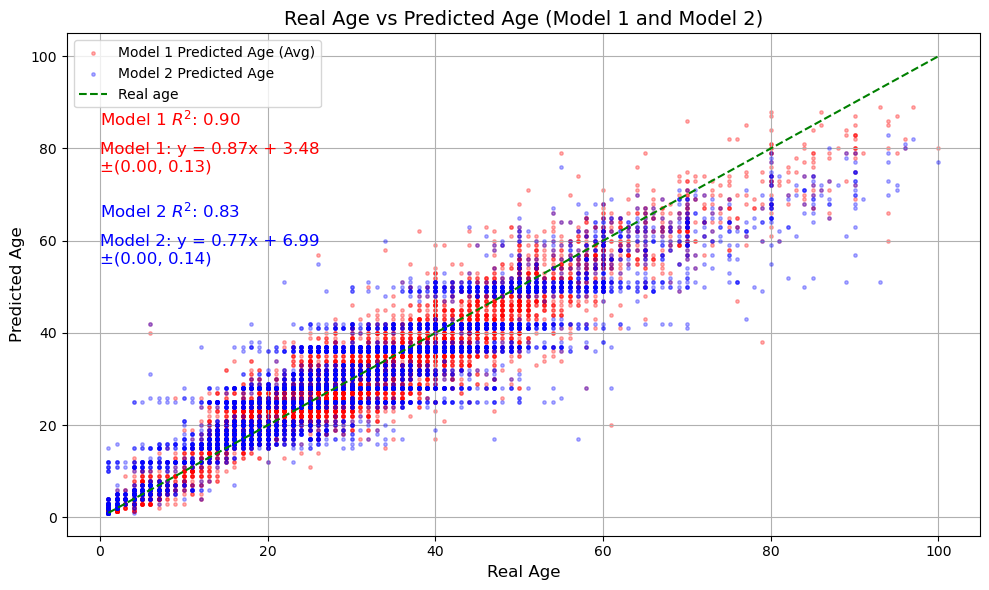
\includegraphics[width=0.7\textwidth]{images/0_Scatter_Real_vs_prediction_Final.png}
    \caption{Scatter plot of predicted age for both models as a function of the real age. The coefficient of determination $R^2$ evaluates how well the predictions from the models (Model 1 and Model 2) align with the actual "real age" value.}
    \label{fig:Scatter}
\end{figure}

\begin{figure}[h]
    \centering
    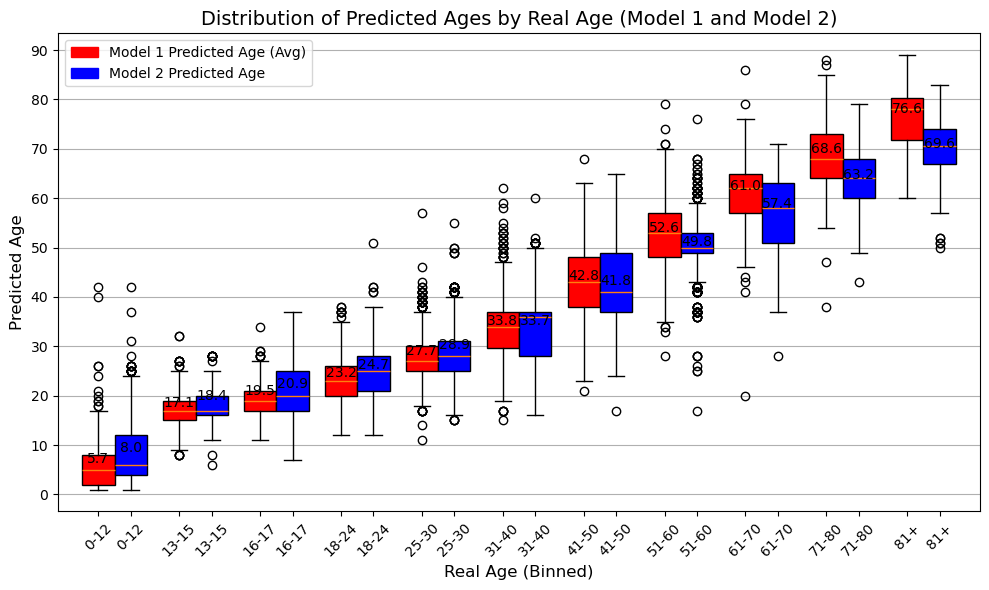
\includegraphics[width=0.7\textwidth]{images/3_Box_Real_vs_prediction_dorpnan_DensePlotGrid.png}
    \caption{Box plot of the average predicted age of Models 1 and 2 as a function of the age bracket. The numbers on the boxes correspond to the model's average.}
    \label{fig:Box}
\end{figure}



Figure~\ref{fig:Box} shows the predicted age of each model across different real age brackets. While both models tend to overestimate the age for younger brackets and underestimate for older ones, Model 1 generally aligns more closely with actual ages.
It is important to note that while the average prediction for certain age brackets may align with true values, this does not necessarily imply strong model performance. The alignment may result from overestimations and underestimations canceling each other out, as suggested by the distribution of errors in Figure~\ref{fig:Scatter}.

%\begin{table}[h]
%\centering
%\begin{tabular}{l|c|c}
%\textbf{Age Bin} & \textbf{Model 1} & \textbf{Model 2} \\ \hline
%0-12    & ok              & ok              \\ 
%13-15   & overestimated   & overestimated   \\ 
%16-17   & overestimated   & overestimated   \\ 
%18-24   & ok              & overestimated   \\ 
%25-30   & ok              & ok              \\ 
%31-40   & ok              & ok              \\ 
%41-50   & ok              & ok              \\ 
%51-60   & ok              & underestimated  \\ 
%61-70   & ok              & underestimated  \\ 
%71-80   & underestimated  & underestimated  \\ 
%81+     & underestimated  & underestimated  \\ 
%\end{tabular}
%\caption{Comparison of Model 1 and Model 2 across different age bins.}
%\label{tab:bars}
%\end{table}

To quantify the models' performance, we evaluate the discrepancy between the true age and predicted values using mean squared error (MSE), mean absolute percentage error (MAPE), and symmetric mean absolute percentage error (SMAPE). MSE emphasizes larger errors, MAPE provides percentage-based insights, and SMAPE offers a symmetric evaluation of errors. As shown in Figure~\ref{fig:metrics}, Model 1 consistently yields lower error rates across all metrics, outperforming Model 2 across all age groups.


\begin{figure}[ht]
    \centering
    \begin{subfigure}{0.32\textwidth}
        \centering
        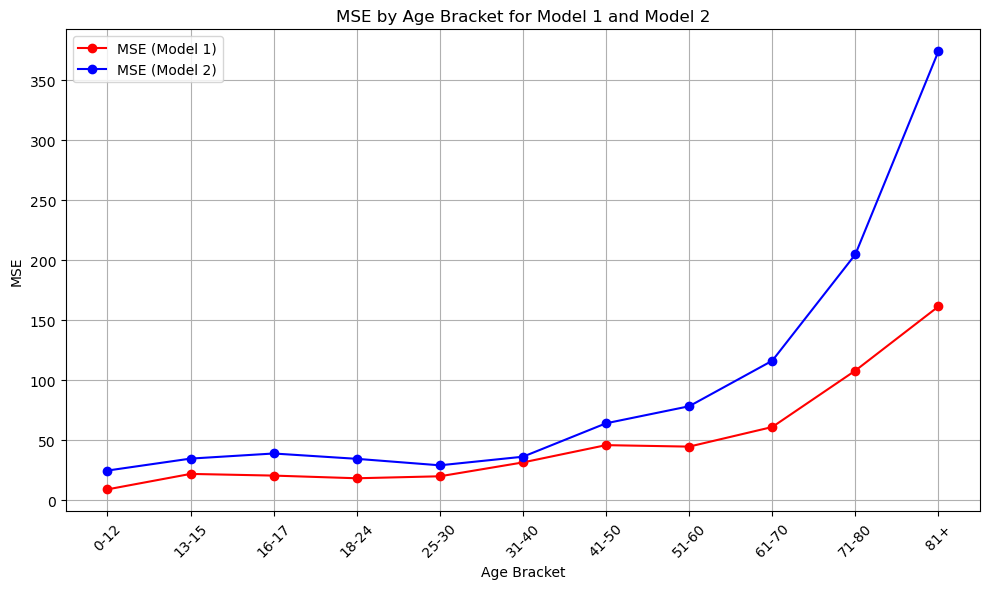
\includegraphics[width=\textwidth]{images/4_MSE.png}
        %\caption{Mean squared error}
        \caption{MSE}
        \label{fig:mse}
    \end{subfigure}
    \hfill
    \begin{subfigure}{0.32\textwidth}
        \centering
        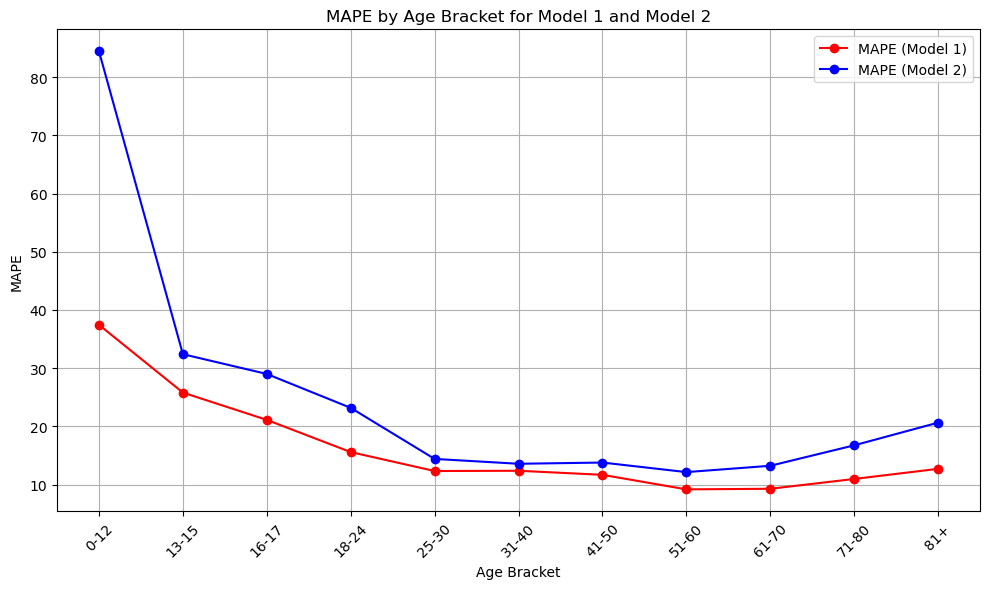
\includegraphics[width=\textwidth]{images/4_MAPE.png}
        %\caption{Mean absolute percentage error}
        \caption{MAPE}
        \label{fig:mape}
    \end{subfigure}
    \hfill
    \begin{subfigure}{0.32\textwidth}
        \centering
        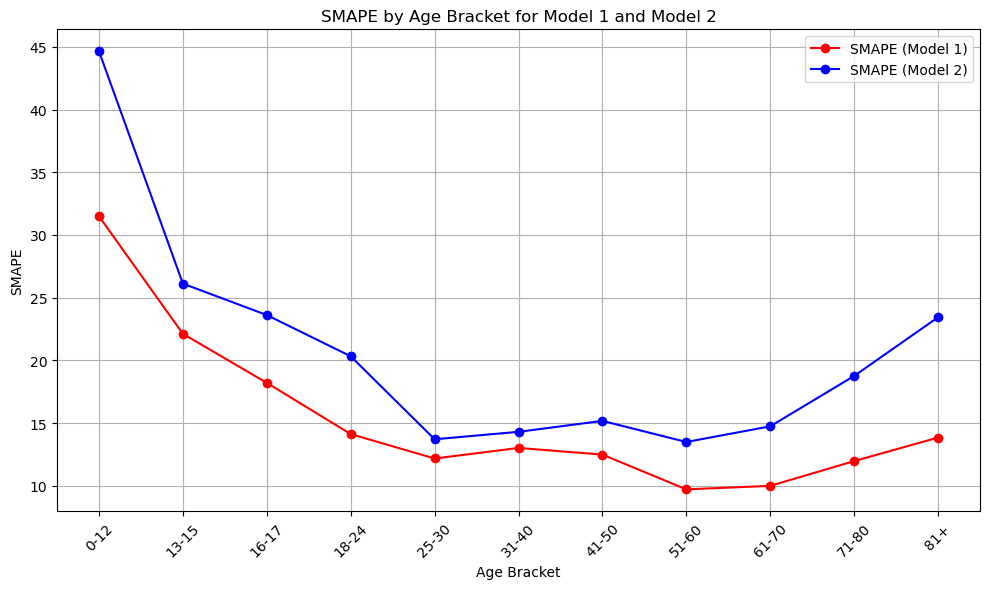
\includegraphics[width=\textwidth]{images/4_SMAPE.png}
        %\caption{Symmetric mean absolute percentage error}
        \caption{SMAPE}
        \label{fig:smape}
    \end{subfigure}
    \caption{Most common metrics to asses the accuracy of a model.}
    \label{fig:metrics}
\end{figure}


%\begin{table}[h]
%\centering
%%\resizebox{\textwidth}{!}{  % This resizes the table to fit the page width
%\begin{tabular}{l|c c| c c| c c}
%\multirow{2}{*}{\textbf{Age Bracket}} & \multicolumn{2}{c}{\textbf{MSE}} & \multicolumn{2}{c}{\textbf{MAPE}}  & \multicolumn{2}{c}{\textbf{SMAPE}} \\ %\cline{2-7} %\hline 
%                             & Model 1    & Model 2    & Model 1     & Model 2    & Model 1     & Model 2     \\ \hline 
%0-12                         & 9.08       & 24.76      & 37.43       & 84.45      & 31.48       & 44.65       \\
%13-15                        & 21.96      & 34.73      & 25.80       & 32.39      & 22.11       & 26.12       \\
%16-17                        & 20.56      & 38.98      & 21.11       & 29.00      & 18.20       & 23.61       \\
%18-24                        & 18.33      & 34.54      & 15.58       & 23.18      & 14.12       & 20.32       \\
%25-30                        & 19.98      & 29.13      & 12.32       & 14.40      & 12.17       & 13.71       \\
%31-40                        & 31.54      & 36.30      & 12.37       & 13.57      & 13.01       & 14.30       \\
%41-50                        & 45.95      & 64.17      & 11.67       & 13.78      & 12.48       & 15.17       \\
%51-60                        & 44.72      & 78.37      & 9.17        & 12.14      & 9.71        & 13.49       \\
%61-70                        & 61.06      & 116.33     & 9.27        & 13.22      & 9.99        & 14.74       \\
%71-80                        & 108.10     & 204.98     & 10.96       & 16.73      & 11.96       & 18.75       \\
%81+                          & 161.57     & 374.38     & 12.70       & 20.63      & 13.84       & 23.43         
%\end{tabular}
%%}
%\caption{Comparison of Model 1 and Model 2 performance across different age brackets using MSE, MAPE, R², and SMAPE.}
%\end{table}



\section{Conclusion}
This analysis demonstrates that both models exhibit similar trends in overestimating younger consumers' ages and underestimating older consumers' ages. However, Model 1, which provides age range predictions, consistently performs better across age groups than Model 2, which directly predicts ages.

Evaluation using MSE, MAPE, and SMAPE metrics confirms that Model 1 achieves lower error rates across all age brackets. Notably, Model 1's performance is less affected by extreme age groups, suggesting greater robustness in diverse age scenarios. Model 2, in contrast, shows significant underestimation for older age groups, which diminishes its utility for personalized experiences in such demographics.

Given these results, Model 1 is recommended for Hanut's age-based customer segmentation. Its superior performance across multiple metrics makes it the more reliable option for age prediction across all age brackers. Future work should focus on refining the models to reduce misestimations at extreme ages and incorporating additional demographic data for improved predictive accuracy.
\end{document}


\section{Error Metrics}

In this analysis, we evaluate the performance of the models using three common error metrics: Mean Squared Error (MSE), Mean Absolute Percentage Error (MAPE), and Symmetric Mean Absolute Percentage Error (SMAPE). These metrics provide different perspectives on model accuracy.

\subsection{Mean Squared Error (MSE)}

The Mean Squared Error (MSE) is a widely used metric that measures the average squared difference between the predicted and actual values. It is defined as:

\[
\text{MSE} = \frac{1}{n} \sum_{i=1}^{n} (y_i - \hat{y}_i)^2
\]

where \( y_i \) represents the actual value, \( \hat{y}_i \) represents the predicted value, and \( n \) is the total number of predictions. MSE gives more weight to larger errors due to the squaring, making it particularly useful when large errors are undesirable.

\subsection{Mean Absolute Percentage Error (MAPE)}

The Mean Absolute Percentage Error (MAPE) measures the average absolute percentage difference between predicted and actual values. It is expressed as:

\[
\text{MAPE} = \frac{100}{n} \sum_{i=1}^{n} \left| \frac{y_i - \hat{y}_i}{y_i} \right|
\]

MAPE provides an intuitive interpretation of model error as a percentage. However, one limitation is that it can be undefined or skewed when actual values are close to zero.

\subsection{Symmetric Mean Absolute Percentage Error (SMAPE)}

The Symmetric Mean Absolute Percentage Error (SMAPE) is a variation of MAPE that addresses its limitations by normalizing the absolute difference between predicted and actual values using the sum of their absolute values. SMAPE is defined as:

\[
\text{SMAPE} = \frac{100}{n} \sum_{i=1}^{n} \frac{|y_i - \hat{y}_i|}{\frac{|y_i| + |\hat{y}_i|}{2}}
\]

This metric ensures that the percentage error is symmetric, meaning that overestimation and underestimation are treated equally, making it a more balanced metric for certain applications.

